\documentclass{beamer}

\usepackage[utf8]{inputenc}
\usepackage[T1]{fontenc}
\usepackage[ngerman]{babel}
\usepackage{graphicx} % Bilder
\usepackage{wrapfig} % Umflussbilder
\usepackage{multicol} % Multiple columns
\usepackage{minted} % Haskell source code
\usepackage{framed} % Frames around source code
\usepackage[framemethod=tikz]{mdframed} % Frames
\usepackage{verbatim} % \begin{comment}...\end{comment}
\usepackage{etoolbox} % manipulate minted
\AtBeginEnvironment{minted}{\fontsize{10}{10}\selectfont}
\AfterEndEnvironment{minted}{}

\mdfdefinestyle{fancy}{
  roundcorner=5pt,
  linewidth=4pt,
  linecolor=red!80,
  backgroundcolor=red!20
}
\newmdenv[style=fancy]{important}

% redifine \em for \emph to use bold instead of italics
\makeatletter
\DeclareRobustCommand{\em}{%
  \@nomath\em \if b\expandafter\@car\f@series\@nil
  \normalfont \else \bfseries \fi}
\makeatother

% Stuff for Beamer
\beamertemplatenavigationsymbolsempty
\usetheme{Warsaw}

\title{Fortgeschrittene Funktionale Programmierung in Haskell}

\begin{document}
  
%----------------------------------------------------------------------------------------  

  \begin{frame}
  \begin{center}
    \huge\textbf{Fortgeschrittene Funktionale Programmierung in Haskell}\\ \bigskip
    \LARGE Universität Bielefeld, Sommersemester 2015\\ \bigskip
    \large Jonas Betzendahl \& Stefan Dresselhaus
    \end{center}
  \end{frame}

%----------------------------------------------------------------------------------------  

\begin{frame}[allowframebreaks]{Outline}
\frametitle{Übersicht}
\tableofcontents
\end{frame}

%----------------------------------------------------------------------------------------
\section*{Alligator Eggs}
%----------------------------------------------------------------------------------------

\begin{frame}

\begin{center}
\Large \textbf{Alligator Eggs} \tiny \bigskip

Idee \& Bilder: Bret Victor\\
\texttt{http://worrydream.com/AlligatorEggs/}
\end{center}

\end{frame}

%----------------------------------------------------------------------------------------
\subsection*{Konzept}

\begin{frame}
Wir betrachten heute ein Spiel, das gleichzeitig bunt und putzig ist und uns erlaubt,
etwas interessantes zu lernen! Es gibt\dots \pause\smallskip

\begin{itemize}
\item \textbf{Hungrige Alligatoren}\\
      
\includegraphics[scale=0.2]{pieces_1.png}\\
      Hungrige Alligatoren sind hungrig! Sie fressen alles, was ihnen vor's Maul kommt.
      Sie bewachen aber außerdem ihre Familien.
      \pause
\item \textbf{Alte Alligatoren}\\
      
\includegraphics[scale=0.2]{pieces_2.png}\\
      Diese Alligatoren haben genug gegessen und bewachen nur noch ihre Familien.
      \pause
\item \textbf{Alligatoreier}\\
      
\includegraphics[scale=0.2]{pieces_3.png}\\
      Aus Eiern schlüpfen demnächst neue Alligatorfamilien.
\end{itemize}

\end{frame}

%----------------------------------------------------------------------------------------

\begin{frame}
\frametitle{Familien}

Alligatoren kommen in Familien daher. Hier ist eine:

\begin{multicols}{2}

\begin{center}

\includegraphics[scale=0.6]{families_1.png} 
\end{center}

\columnbreak
\pause

Hier ist noch nicht viel zu sehen, was wirklich interessiert.\smallskip\smallskip

Nur ein grüner Alligator, der sein grünes Ei bewacht.\\Ist er nicht süß?

\end{multicols}

\end{frame}

%----------------------------------------------------------------------------------------

\begin{frame}
\frametitle{Familien}

Hier ist eine weitere Familie, dieses Mal mit mehr Mitgliedern.\pause

\begin{multicols}{2}

\begin{center}
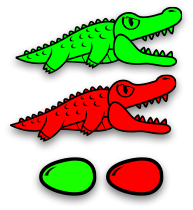
\includegraphics[scale=0.6]{families_2.png} 
\end{center}

\columnbreak

Ein grüner und ein roter Alligator bewachen ein grünes und ein rotes Ei.\bigskip

Oder anders formuliert:

Ein grüner Alligator bewacht einen roten Alligator und der rote Alligator bewacht die zwei Eier.

\end{multicols}

\end{frame}

%----------------------------------------------------------------------------------------

\begin{frame}
\frametitle{Familien}

Dieses Mal haben wir eine richtige Großfamilie:\pause

\begin{multicols}{2}

\begin{center}
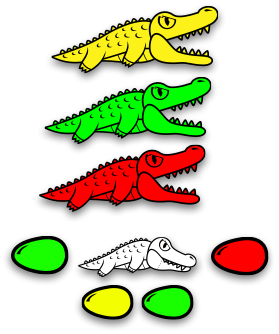
\includegraphics[scale=0.5]{families_3.png} 
\end{center}

\columnbreak
\pause

Hier haben wir drei hungrige Alligatoren, die Wache halten. Einen gelben, einen grünen und einen roten.\pause\bigskip

Sie bewachen drei Dinge: Ein grünes Ei, einen alten Alligator und ein rotes Ei.\pause\bigskip

Der alte Alligator hingegen bewacht ein gelbes und ein grünes Ei. 

\end{multicols}

\end{frame}


%----------------------------------------------------------------------------------------
\subsection*{Die Essensregel}

%----------------------------------------------------------------------------------------
\subsection*{Die Farbenregel}

%----------------------------------------------------------------------------------------
\section*{Der Lambda-Würfel}
%----------------------------------------------------------------------------------------

%----------------------------------------------------------------------------------------
\section*{Recursion Schemes}
%----------------------------------------------------------------------------------------

%----------------------------------------------------------------------------------------

\end{document}